\begin{exercice}
   \begin{enumerate}
      \item Le triangle ci-dessous a été réalisé à main levée.\\
      Construire ce triangle avec les instruments de géométrie en respectant les mesures indiquées.\\
      Puis placer le point $I$ milieu de $[HG]$, tracer le segment $[IF]$ et mesurer la longueur de ce segment.
      \begin{center}
         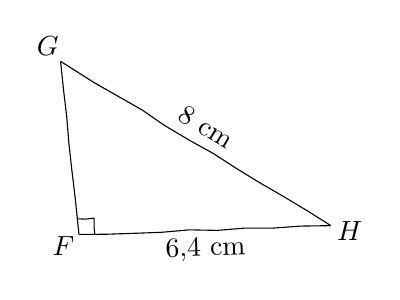
\begin{tikzpicture}[baseline,scale = 0.5]
            \tikzset{
               point/.style={
               thick,
               draw,
               cross out,
               inner sep=0pt,
               minimum width=5pt,
               minimum height=5pt,
               },
            }
            \draw [color={black}] (3.215500394812357,-0.3880170240615448) node[anchor = center, rotate = -358] {6,4 cm};
            \draw [color={black}] (3.2240774719085015,2.7374299425741384) node[anchor = center, rotate = -31.3] {8 cm};
            \draw[color={black},decorate,decoration={random steps , segment length=3pt, amplitude = 0.3pt}] (0.39975633080763834,0.013959798681000389)--(0.38579653212663795,0.41371612948863873)--(-0.042291482531377246,0.3977580049543921);
            \draw[color ={black},decorate,decoration={random steps , amplitude = 0.3pt}] (0,0)--(6.396101292922213,0.22335677889600622);
            \draw[color ={black},decorate,decoration={random steps , amplitude = 0.3pt}] (6.396101292922213,0.22335677889600622)--(-0.46751758417200406,4.397075969691659);
            \draw[color ={black},decorate,decoration={random steps , amplitude = 0.3pt}] (-0.46751758417200406,4.397075969691659)--(0,0);
            \draw [color={black}] (-0.3943757249995441,-0.30735612492853326) node[anchor = center,scale=1] {$F$};
            \draw [color={black}] (6.875287623071181,0.08059662689844949) node[anchor = center,scale=1] {$H$};
            \draw [color={black}] (-0.7925231268719926,4.777038332583413) node[anchor = center,scale=1] {$G$};
         \end{tikzpicture}
      \end{center}
      \item Le triangle ci-dessous a été réalisé à main levée.\\
      Construire ce triangle avec les instruments de géométrie en respectant les mesures indiquées.\\
      Puis placer le point $O$ milieu de $[NL]$, tracer le segment $[OM]$ et mesurer la longueur de ce segment.
      \begin{center}
         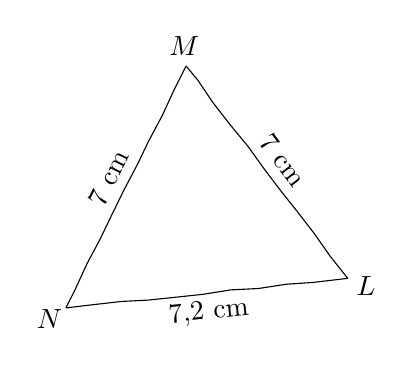
\begin{tikzpicture}[baseline,scale = 0.5]
            \tikzset{
               point/.style={
               thick,
               draw,
               cross out,
               inner sep=0pt,
               minimum width=5pt,
               minimum height=5pt,
               },
            }
            \draw [color={black}] (3.6325430549596107,-0.12095847992058423) node[anchor = center, rotate = -354] {7,2 cm};
            \draw [color={black}] (5.504446528655759,3.7526035625970087) node[anchor = center, rotate = -52.71] {7 cm};
            \draw [color={black}] (1.0785671446003247,3.295778527288993) node[anchor = center, rotate = 63.59] {7 cm};
            \draw[color ={black},decorate,decoration={random steps , amplitude = 0.3pt}] (0,0)--(7.160557646651568,0.752604935527105);
            \draw[color ={black},decorate,decoration={random steps , amplitude = 0.3pt}] (7.160557646651568,0.752604935527105)--(3.0527597122408525,6.146747992615375);
            \draw[color ={black},decorate,decoration={random steps , amplitude = 0.3pt}] (3.0527597122408525,6.146747992615375)--(0,0);
            \draw [color={black}] (-0.41432340982180227,-0.27988589116573026) node[anchor = center,scale=1] {$N$};
            \draw [color={black}] (7.622873190856785,0.5621729592567468) node[anchor = center,scale=1] {$L$};
            \draw [color={black}] (3.0072408217399547,6.644671712282923) node[anchor = center,scale=1] {$M$};
         \end{tikzpicture}
      \end{center}
      \item Le triangle ci-dessous a été réalisé à main levée.\\
      Construire ce triangle avec les instruments de géométrie en respectant les mesures indiquées.\\
      Puis placer le point $N$ milieu de $[ML]$, tracer le segment $[NK]$ et mesurer la longueur de ce segment.
      \begin{center}
         \begin{tikzpicture}[baseline,scale = 0.5]
            \tikzset{
               point/.style={
               thick,
               draw,
               cross out,
               inner sep=0pt,
               minimum width=5pt,
               minimum height=5pt,
               },
            }
            \draw [color={black}] (5.2,-0.5) node[anchor = center, rotate = 0] {10,4 cm};
            \draw [color={black}] (8.385734266837742,4.598557809390308) node[anchor = center, rotate = -60.63] {10,4 cm};
            \draw [color={black}] (2.32727865819191,4.62036518223622) node[anchor = center, rotate = 57.72] {10,4 cm};
            \draw[color ={black},decorate,decoration={random steps , amplitude = 0.3pt}] (0,0)--(10.4,0);
            \draw[color ={black},decorate,decoration={random steps , amplitude = 0.3pt}] (10.4,0)--(5.5,8.706664199358162);
            \draw[color ={black},decorate,decoration={random steps , amplitude = 0.3pt}] (5.5,8.706664199358162)--(0,0);
            \draw [color={black}] (-0.4385536957117573,-0.24014715483960813) node[anchor = center,scale=1] {$M$};
            \draw [color={black}] (10.834563702832583,-0.24729413292764457) node[anchor = center,scale=1] {$L$};
            \draw [color={black}] (5.517217964618122,9.206367653112896) node[anchor = center,scale=1] {$K$};
         \end{tikzpicture}
      \end{center}
   \end{enumerate}
\end{exercice}
 
\begin{corrige}
   \begin{enumerate}
      \item Voici la construction que tu devais réaliser.\\
      Pour cette construction, nous avons utilisé la règle graduée, l'équerre et le compas.\\
      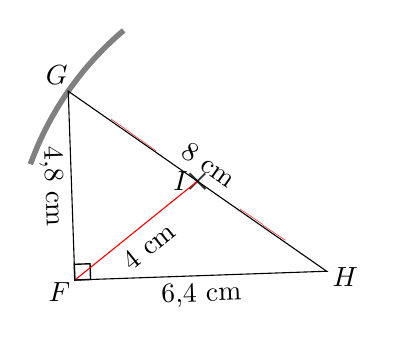
\begin{tikzpicture}[baseline,scale=0.5]
         \tikzset{
            point/.style={
            thick,
            draw,
            cross out,
            inner sep=0pt,
            minimum width=5pt,
            minimum height=5pt,
            },
         }
         \draw[color={gray},line width = 2] (1.2398979391472595,6.340019837665871) arc (130.13:160.13:8) ;
         \draw[color={black},line width = 0.5] (0,0)--(0.39975633080763834,0.013959798681000389)--(0.38579653212663795,0.41371612948863873)--(-0.013959798681000342,0.3997563308076383)--cycle;
         \draw [color={black}] (3.215500394812357,-0.3880170240615448) node[anchor = center, rotate = -358] {6,4 cm};
         \draw [color={black}] (3.4001493037998327,2.9204425541122214) node[anchor = center, rotate = -34.87] {8 cm};
         \draw [color={black}] (-0.5834542055955498,2.381088236494579) node[anchor = center, rotate = -88] {4,8 cm};
         \draw (3.1142918543751046,2.5102163742938326) node[left] {$I$};
         \draw[color ={{black}},line width = 0.6666666666666666,opacity = 0.8] (2.9142918543751044,2.7102163742938328)--(3.3142918543751048,2.3102163742938324);
         \draw[color ={{black}},line width = 0.6666666666666666,opacity = 0.8] (2.9142918543751044,2.3102163742938324)--(3.3142918543751048,2.7102163742938328);
         \draw[color ={red}] (3.1142918543751046,2.5102163742938326)--(0,0);
         \draw [color={red}] (1.4733871351015502,3.6536461719927456) node[anchor = center, rotate = -35] {||};
         \draw [color={red}] (4.755196573648659,1.3667865765949194) node[anchor = center, rotate = -34] {||};
         \draw [color={black}] (1.8709229739742814,0.8658217053500282) node[anchor = center, rotate = -321.13] {4 cm};
         \draw[color={black}] (0,0)--(6.396101292922213,0.22335677889600622)--(-0.16751758417200407,4.797075969691659)--cycle;
         \draw [color={black}] (-0.38928648179688796,-0.31377704678672913) node[anchor = center,scale=1] {$F$};
         \draw [color={black}] (6.870107704184575,0.06424071408111232) node[anchor = center,scale=1] {$H$};
         \draw [color={black}] (-0.4592177963503765,5.203168306747029) node[anchor = center,scale=1] {$G$};
      \end{tikzpicture}
      
      {\red Auto-vérification : le segment $[IF]$ mesure environ 4 cm}.
      \item Voici la construction que tu devais réaliser.\\
      Pour cette construction, nous avons utilisé le compas et la règle graduée.\\
      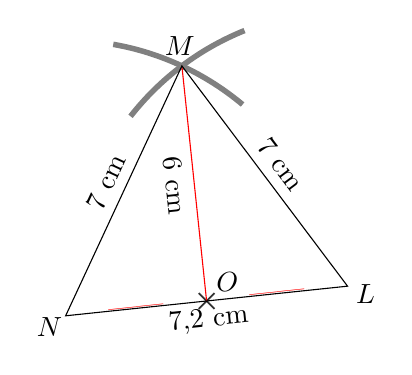
\begin{tikzpicture}[baseline,scale=0.5]
         \tikzset{
            point/.style={
            thick,
            draw,
            cross out,
            inner sep=0pt,
            minimum width=5pt,
            minimum height=5pt,
            },
         }
         \draw[color={gray},line width = 2] (4.494806119834369,5.366257349876121) arc (50.05:80.05:6.999999999999999) ;
         \draw[color={gray},line width = 2] (4.544007714200945,7.245190433692888) arc (111.95:141.95:6.999999999999998) ;
         \draw [color={black}] (3.6325430549596107,-0.12095847992058423) node[anchor = center, rotate = -354] {7,2 cm};
         \draw [color={black}] (5.456240326381087,3.850233459386291) node[anchor = center, rotate = -53.05] {7 cm};
         \draw [color={black}] (1.0230407137907565,3.3842854043248916) node[anchor = center, rotate = 65.05] {7 cm};
         \draw (3.580278823325784,0.3763024677635525) node[above right] {$O$};
         \draw[color ={{black}},line width = 0.6666666666666666,opacity = 0.8] (3.3802788233257837,0.5763024677635524)--(3.780278823325784,0.17630246776355246);
         \draw[color ={{black}},line width = 0.6666666666666666,opacity = 0.8] (3.3802788233257837,0.17630246776355246)--(3.780278823325784,0.5763024677635524);
         \draw[color ={red}] (3.580278823325784,0.3763024677635525)--(2.9527597122408524,6.346747992615375);
         \draw [color={red}] (5.3704182349886755,0.5644537016453287) node[anchor = center, rotate = 6] {||};
         \draw [color={red}] (1.790139411662892,0.18815123388177624) node[anchor = center, rotate = -354] {||};
         \draw [color={black}] (2.769258320099181,3.309260998555637) node[anchor = center, rotate = -84] {6 cm};
         \draw[color={black}] (0,0)--(7.160557646651568,0.752604935527105)--(2.9527597122408524,6.346747992615375)--cycle;
         \draw [color={black}] (-0.40923480644233434,-0.28727490874788364) node[anchor = center,scale=1] {$N$};
         \draw [color={black}] (7.6205775027171905,0.5566923733332438) node[anchor = center,scale=1] {$L$};
         \draw [color={black}] (2.9004954806070256,6.844008940299512) node[anchor = center,scale=1] {$M$};
      \end{tikzpicture}
      
      {\red Auto-vérification : le segment $[OM]$ mesure environ 6 cm}.
      \item Voici la construction que tu devais réaliser.\\
      Pour cette construction, nous avons utilisé le compas et la règle graduée.\\
      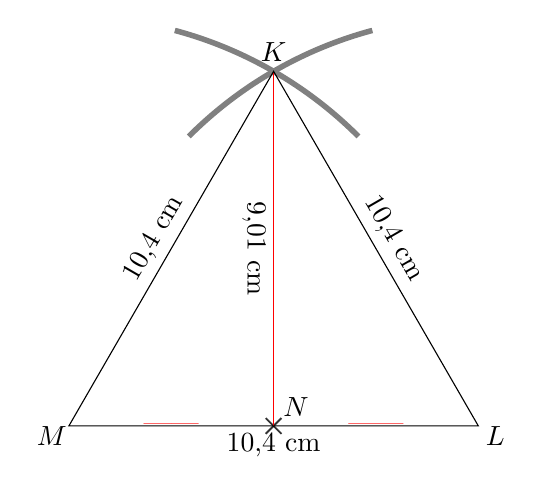
\begin{tikzpicture}[baseline,scale=0.5]
         \tikzset{
            point/.style={
            thick,
            draw,
            cross out,
            inner sep=0pt,
            minimum width=5pt,
            minimum height=5pt,
            },
         }
         \draw[color={gray},line width = 2] (7.353910524340095,7.353910524340096) arc (45:75:10.4) ;
         \draw[color={gray},line width = 2] (7.708281930933784,10.045628593406311) arc (105:135:10.4) ;
         \draw [color={black}] (5.2,-0.5) node[anchor = center, rotate = 0] {10,4 cm};
         \draw [color={black}] (8.23301270189222,4.753332099679081) node[anchor = center, rotate = -60] {10,4 cm};
         \draw [color={black}] (2.166987298107781,4.753332099679081) node[anchor = center, rotate = 60] {10,4 cm};
         \draw (5.2,0) node[above right] {$N$};
         \draw[color ={{black}},line width = 0.6666666666666666,opacity = 0.8] (5,0.2)--(5.4,-0.2);
         \draw[color ={{black}},line width = 0.6666666666666666,opacity = 0.8] (5,-0.2)--(5.4,0.2);
         \draw[color ={red}] (5.2,0)--(5.2,9.006664199358163);
         \draw [color={red}] (7.800000000000001,0) node[anchor = center, rotate = 0] {||};
         \draw [color={red}] (2.6,0) node[anchor = center, rotate = 0] {||};
         \draw [color={black}] (4.7,4.503332099679081) node[anchor = center, rotate = -90] {9,01 cm};
         \draw[color={black}] (0,0)--(10.4,0)--(5.2,9.006664199358163)--cycle;
         \draw [color={black}] (-0.43301270189221963,-0.25) node[anchor = center,scale=1] {$M$};
         \draw [color={black}] (10.833012701892219,-0.25) node[anchor = center,scale=1] {$L$};
         \draw [color={black}] (5.2,9.506664199358163) node[anchor = center,scale=1] {$K$};
      \end{tikzpicture}
      
      {\red Auto-vérification : le segment $[NK]$ mesure environ 9,01 cm}.
   \end{enumerate}

\end{corrige}
